% This is file JFM2esam.tex
% first release v1.0, 20th October 1996
%       release v1.01, 29th October 1996
%       release v1.1, 25th June 1997
%       release v2.0, 27th July 2004
%       release v3.0, 16th July 2014
%   (based on JFMsampl.tex v1.3 for LaTeX2.09)
% Copyright (C) 1996, 1997, 2014 Cambridge University Press

\documentclass{jfm}
\usepackage{graphicx}
\usepackage{epstopdf, epsfig}

\newtheorem{lemma}{Lemma}
\newtheorem{corollary}{Corollary}

\shorttitle{Guidelines for authors}
\shortauthor{A. N. Other, H.-C. Smith and J. Q. Public}

\title{Guidelines for authors and submission template}

\author{Alan N. Other\aff{1}
  \corresp{\email{jfm@damtp.cam.ac.uk}},
  H. - C. Smith\aff{1}
 \and J. Q.  Public\aff{2}}

\affiliation{\aff{1}Department of Chemical Engineering, University of America,
Somewhere, IN 12345, USA
\aff{2}Department of Aerospace and Mechanical Engineering, University of
Camford, Academic Street, Camford CF3 5QL, UK}

\begin{document}

\maketitle

\begin{abstract}
This file contains instructions for authors planning to submit a paper to the {\it Journal of Fluid Mechanics}. These instructions were generated in {\LaTeX} using the JFM style, so the {\LaTeX} source file can be used as a template for submissions. The present paragraph appears in the \verb}abstract} environment. All papers should feature a single-paragraph abstract of no more than 250 words, which provides a summary of the main aims and results. 
\end{abstract}

\begin{keywords}
Authors should not enter keywords on the manuscript, as these must be chosen by the author during the online submission process and will then be added during the typesetting process (see http://journals.cambridge.org/data/\linebreak[3]relatedlink/jfm-\linebreak[3]keywords.pdf for the full list)
\end{keywords}

\section{How to submit to the \textbf{\textit{Journal of Fluid Mechanics}}}
Authors must submit using the online submission and peer review system, Scholar One Manuscripts (formerly Manuscript Central) at http://mc.manuscriptcentral.com/jfm. If visiting the site for the first time, users must create a new account by clicking on `register here'. Once logged in, authors should click on the `Corresponding Author Centre', from which point a new manuscript can be submitted, with step-by-step instructions provided. Authors must at this stage specify whether the submission is a standard paper, or a {\it JFM Rapids} paper (see \S\ref{sec:filetypes} for more details). In addition, authors must specify an editor to whom the paper will be submitted from the drop-down list provided. Note that all editors exclusively deal with either standard papers or {\it JFM Rapids} (clearly indicated on the list), so please ensure that you choose an editor accordingly. Once your submission is completed you will receive an email confirmation.  Book reviews should not be submitted via the online submission site and should instead be submitted by email to c.p.caulfield@damtp.cam.ac.uk.
 
\section{Rules of submission}\label{sec:rules_submission}
Submission of a paper implies a declaration by the author that the work has not previously been published, that it is not being considered for publication elsewhere and that it has not already been considered by a different editor of the Journal. Note that a report on a conference must be submitted within 3 months of the meeting.

\section{Types of paper}\label{sec:types_paper}
\subsection{Standard papers}
Regular submissions to JFM are termed `standard papers'. Note that such papers must contain original research, as review articles are not published in JFM. Papers should be written in a concise manner; though JFM has no page limit, each paper will be judged on its own merits, and those deemed excessive in length will be rejected or will require significant revision.  
\subsection{JFM Rapids}
{\it JFM Rapids} is devoted to the rapid publication of short, high-impact papers across the full range of fluid mechanics. Manuscripts submitted as {\it Rapids}  must be strictly 10 or fewer printed pages, and must be submitted in {\LaTeX} using the jfm.cls class file, so as to ensure that they meet the page limit and to expedite their production.  The principal and over-riding objective is to publish papers of the highest scientific quality. 

Once a paper is submitted, referees are asked to provide reports with a short turnaround.  In order to be accepted for publication in {\it JFM Rapids}, such papers must require only minor revisions to improve clarity, usually without recourse to a second round of refereeing. In this case, and at the discretion of the editor, some additional pages may be allowed to address specific points raised by the referees, such as the addition of an extra figure or some explanatory text.  

In cases where the editor, guided by the referees, judges that a paper has merit but requires substantial revision that will require significant refereeing, a decision of `revise and resubmit' will be given. On re-submission, such papers will be handled as standard JFM papers and if accepted will not subsequently appear as {\it JFM Rapids}.

{\it Rapids} will be published online within one month of final acceptance.  They will appear within a designated section on the Journal of Fluid Mechanics website.  Each {\it Rapid} will be cited and indexed as a JFM article but with a distinctive {\it Rapids} identifier, and will be assigned to a JFM volume. {\it Rapids} will not be included in the regular print versions of JFM, and accordingly they incur no colour figure charges.
 
\section{File types}\label{sec:filetypes}
Authors are strongly encouraged to compose their papers in {\LaTeX}, using the jfm.cls style file and supporting files provided at http://journals.cambridge.org/images/\linebreak[4]fileUpload/documents/jfm-ifc.zip, with the jfm-instructions.tex file serving as a template (note that this is mandatory for {\it JFM Rapids}). A PDF of the {\LaTeX} file should then be generated and submitted via the submission site. Please note that PDFs larger than 3MB are not acceptable for review. There is no need to submit the {\LaTeX} source file alongside the PDF, but upon provisional acceptance of the paper, the {\LaTeX} source file, along with individual figure files and a PDF of the final version, will need to be submitted for typesetting purposes. 
Authors may also compose standard papers in Word, though this will lead to the paper spending a longer period in production. If using Word, please note that equations must NOT be converted to picture format and the file must be saved with the option `make equation editable'. 
\section{Preparing your manuscript}
Authors should write their papers clearly and concisely in English, adhering to JFM's established style for notation, as provided in \S\ref{notstyle}. We encourage the submission of online supplementary material alongside the manuscript where appropriate (see section \ref{online}). Metric units should be used throughout and all abbreviations must be defined at first use, even those deemed to be well known to the readership. British spelling must be used, and should follow the \textit{Shorter Oxford English Dictionary}.

\subsection{Figures}
Figures should be as small as possible while displaying clearly all the information required, and with all lettering readable. Every effort should be taken to avoid figures that run over more than one page. Figures submitted in colour will appear online in colour but, with the exception of {\it JFM Rapids}, all figures will be printed in black and white unless authors specify during submission that figures should be printed in colour, for which there is a charge of \pounds200 per figure with a cap of \pounds1000 per article plus taxes where applicable (colour is free for {\it JFM Rapids}).  Note that separate figures for online and print will {\bf not} be accepted and it is the author's responsibility to ensure that if a figure is to appear in colour online only, that same figure will still be meaningful when printed in black and white (for example, do not rely upon colours to distinguish lines if those colours will just appear as similar shades of grey when printed). If using colour, authors should also ensure that some consistency is applied within the manuscript. For review purposes figures should be embedded within the manuscript. Upon final acceptance, however, individual figure files will be required for production. These should be submitted in EPS or high-resolution TIFF format (1200 dpi for lines, 300 dpi for halftone and colour in CMYK format, and 600 dpi for a mixture of lines and halftone). The minimum acceptable width of any line is 0.5pt. Each figure should be accompanied by a single caption, to appear beneath, and must be cited in the text. Figures should appear in the order in which they are first mentioned in the text and figure files must be named accordingly (`Figure 1.eps', `Figure 2a.tiff', etc) to assist the production process (and numbering of figures should continue through any appendices). The word \textit {figure} is only capitalized at the start of a sentence. For example see figures \ref{fig:ka} and \ref{fig:kd}. Failure to follow figure guidelines may result in a request for resupply and a subsequent delay in the production process. Note that {\em all} figures are relabelled by the typesetter, so please ensure all figure labels are carefully checked against your originals when you receive your proofs.

\begin{figure}
  \centerline{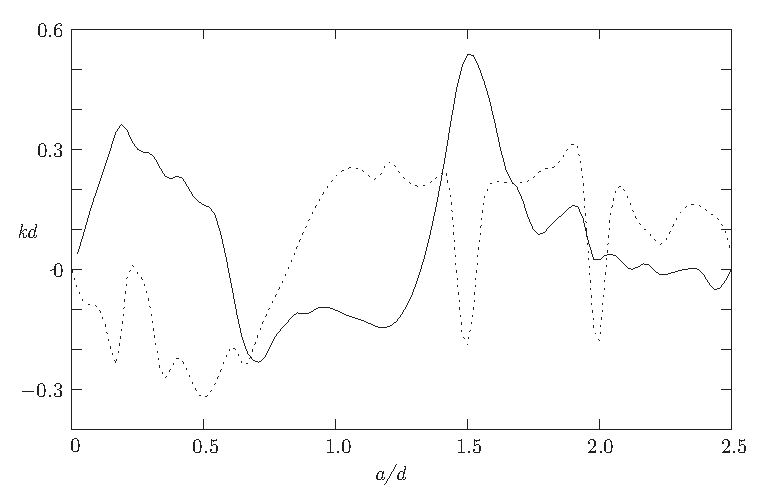
\includegraphics{trapped}}% Images in 100% size
  \caption{Trapped-mode wavenumbers, $kd$, plotted against $a/d$ for
    three ellipses:\protect\\
    ---$\!$---,
    $b/a=1$; $\cdots$\,$\cdots$, $b/a=1.5$.}
\label{fig:ka}
\end{figure}

\begin{figure}
  \centerline{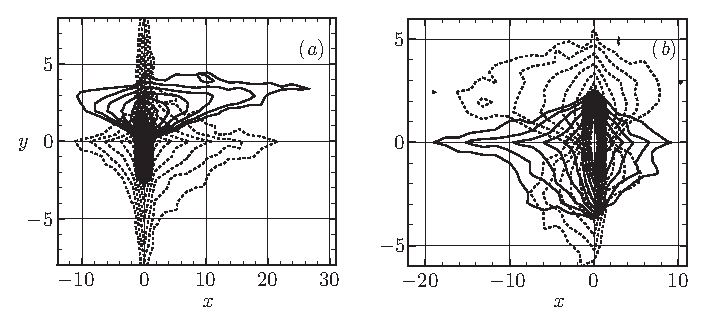
\includegraphics{modes}}
  \caption{The features of the four possible modes corresponding to
  (\textit{a}) periodic\protect\\ and (\textit{b}) half-periodic solutions.}
\label{fig:kd}
\end{figure}

\subsection{Tables}
Tables, however small, must be numbered sequentially in the order in which they are mentioned in the text. The word \textit {table} is only capitalized at the start of a sentence. See table \ref{tab:kd} for an example.

\begin{table}
  \begin{center}
\def~{\hphantom{0}}
  \begin{tabular}{lccc}
      $a/d$  & $M=4$   &   $M=8$ & Callan \etal \\[3pt]
       0.1   & 1.56905 & ~~1.56~ & 1.56904\\
       0.3   & 1.50484 & ~~1.504 & 1.50484\\
       0.55  & 1.39128 & ~~1.391 & 1.39131\\
       0.7   & 1.32281 & ~10.322 & 1.32288\\
       0.913 & 1.34479 & 100.351 & 1.35185\\
  \end{tabular}
  \caption{Values of $kd$ at which trapped modes occur when $\rho(\theta)=a$}
  \label{tab:kd}
  \end{center}
\end{table}

\subsection{Online supplementary material}\label{online}
Relevant material which is not suitable for print production, such as movies or numerical simulations/animations, can be uploaded as part of the initial submission. Movies should be designated as `Movie' and each individual file must be accompanied by a separate caption and a suitable title (eg Movie 1). Accepted formats are .mov, .mpg, .mp4, and .avi, though they should be archived as a .zip or .tar file before uploading. Each movie should be no more than 10MB. Upon publication these materials will then be hosted online alongside the final published article. Likewise, should there be detailed mathematical relations, tables or figures which are likely to be useful only to a few specialists or take up excessive space in the printed journal, these can also be published online as supplementary material [designated as `Other supplementary material']. Note that supplementary material is published `as is', with no further production performed.

\section{Editorial decisions}
\subsection{Revision}
If a revision is requested, you should upload revised files following the same procedure as for submitting a new paper. You begin by clicking on `Manuscripts with decision' in your Corresponding Author Center, and then on `Create a revision'. (Note that if you abandon the process before completing the submission, to continue the submission, you must click on `Revised manuscripts in draft'.) There is a new first page showing the decision letter and a space for your reply to the referee's/editor's comments. You also have the opportunity at this stage to upload your reply to the comments as a separate file. All the values filled in on original submission are displayed again. The ID number of the paper will be appended `.R1'. Also note that if a manuscript is submitted as a {\it JFM Rapid}, but requires substantial revision, it will be re-designated as a standard paper, and the ID and paper type will be amended to reflect this.

\subsection{Provisional acceptance}
If the paper is accepted as suitable for publication you will be sent a provisional acceptance decision. This enables you to upload the final files required for production:
(1) the final PDF or word version of the paper, designated as a `main document';
(2) any source files (see section \ref{sec:filetypes}) which must be designated as `production (not for review)' and uploaded as a single .zip or .tar file.

\subsection{Acceptance}
On receipt of the production files you will be sent an email indicating completion of the acceptance process.

\section{Publication process}
Once a paper has been accepted for publication and the source files have been uploaded, the manuscript will be sent to Cambridge University Press for copyediting and typesetting, and will be assigned a digital object identifier (doi). When the proof is ready, authors will receive an email alert containing a link to the PDF of the proof, and instructions for its correction and return. It is imperative that authors check their proofs closely, particularly the equations and figures, which should be checked against the accepted file, as the production schedule does not allow for corrections at a later stage. Once ready for printing, papers will be published online on Cambridge Journals Online in the current `open' volume. {\it JFM Rapids} will also be assigned to the current open volume, but will receive an article number in place of traditional pagination, as they will not appear in the print version of that volume. Each volume will be kept open for approximately two weeks, at which point it will be considered `closed', and then printed and distributed. The following volume will be immediately opened. Note that the PDF published online is the Version of Record, matching the print version, and no further alterations/corrections to this document will be allowed. The corresponding author is emailed a link to the published article when it is first published online.

\section{Obtaining help}
Technical support for the online submission system is available by clicking on the `Get Help Now' link at the top-right corner of each page of the submission site. Any other questions relating to the submission or publication process should be directed to the JFM Editorial Assistant, Mrs Amanda Johns, at ajohns@cambridge.org.

\section{Notation and style}\label{notstyle}
Generally any queries concerning notation and journal style can be answered by viewing recent pages in the Journal. However, the following guide provides the key points to note. It is expected that Journal style will be followed, and authors should take care to define all variables or entities upon first use. Also note that footnotes are not normally accepted.

\subsection{Mathematical notation}
\subsubsection{Setting variables, functions, vectors, matrices etc}
{\bf Italic font} should be used for denoting variables, with multiple-letter symbols avoided except in the case of dimensionless numbers such as $\Rey$, $\Pran$ and $\Pen$ (Reynolds, Prandtl, and P\'eclet numbers respectively, which are defined as \verb}\Rey}, \verb}\Pran} and {\verb}\Pen} in the template).\\
{\bf Upright Roman font} (or upright Greek where appropriate) should be used for:\\
Operators: sin, log, d, $\Delta$, e etc.\\
Constants: i ($\sqrt{-1}$), $\upi$ (defined as \verb}\upi}), etc.\\
Functions: $\Ai$, $\Bi$ (Airy functions, defined as \verb}\Ai} and \verb}\Bi}), $\Real$ (real part, defined as \verb}\Real}), $\Imag$ (imaginary part, defined as \verb}\Imag}), etc.\\
Physical units: cm, s, etc\\
Abbreviations: c.c. (complex conjugate), h.o.t. (higher-order terms), DNS, etc.\\
{\bf Bold italic font} (or bold sloping Greek) should be used for:\\
Vectors (with the centred dot for a scalar product also in bold): $\boldsymbol{i \cdot j}$\\
{\bf Bold sloping sans serif font}, defined by the \verb}\mathsfbi} macro, should be used for:\\
Tensors and matrices: $\mathsfbi{D}$ \\
{\bf Script font} (for example $\mathcal{G}$, $\mathcal{R}$) can be used as an alternative to italic when the same letter denotes a different quantity (use \verb}\mathcal} in \LaTeX)\\
The product symbol ($\times$) should only be used to denote multiplication where an equation is broken over more than one line, to denote a cross product, or between numbers (the $\cdot$ symbol should not be used, except to denote a scalar product specifically).\\ 

\subsubsection{Other symbols}
A centred point should be used only for the scalar product of vectors.
Large numbers that are not scientific powers should not include commas, but have the
form 1600 or 16 000 or 160 000.
Use \textit{O} to denote `of the order of', not the \LaTeX\ $\mathcal{O}$.

\section{Citations and references}
All papers included in the References section must be cited in the article, and vice versa. Citations should be included as, for example ``It has been shown \citep{Rogallo81} that...'' (using the {\verb}\citep} command, part of the natbib package) ``recent work by \citet{Dennis85}...'' (using {\verb}\citet}).
The natbib package can be used to generate citation variations, as shown below.\\
\verb#\citet[pp. 2-4]{Hwang70}#:\\
\citet[pp. 2-4]{Hwang70} \\
\verb#\citep[p. 6]{Worster92}#:\\
\citep[p. 6]{Worster92}\\
\verb#\citep[see][]{Koch83, Lee71, Linton92}#:\\
\citep[see][]{Koch83, Lee71, Linton92}\\
\verb#\citep[see][p. 18]{Martin80}#:\\
\citep[see][p. 18]{Martin80}\\
\verb#\citep{Brownell04,Brownell07,Ursell50,Wijngaarden68,Miller91}#:\\
\citep{Brownell04,Brownell07,Ursell50,Wijngaarden68,Miller91}\\
The References section can either be built from individual \verb#\bibitem# commands, or can be built using BibTex. The BibTex files used to generate the references in this document can be found in the zip file at http://journals.cambridge.org/\linebreak[3]data/\linebreak[3]relatedlink/\linebreak[3]jfm-ifc.zip.\\

Acknowledgements should be included at the end of the paper, before the References section or any appendicies, and should be a separate paragraph without a heading. Several anonymous individuals are thanked for contributions to these instructions.

\appendix
\section{}\label{appA}
This appendix contains sample equations in the JFM style. Please refer to the {\LaTeX} source file for examples of how to display such equations in your manuscript.

\begin{equation}
  (\nabla^2+k^2)G_s=(\nabla^2+k^2)G_a=0
  \label{Helm}
\end{equation}

\begin{equation}
  \bnabla\bcdot\boldsymbol{v} = 0,\quad \nabla^{2}P=
    \bnabla\bcdot(\boldsymbol{v}\times \boldsymbol{w}).
\end{equation}

\begin{equation}
  G_s,G_a\sim 1 / (2\upi)\ln r
  \quad \mbox{as\ }\quad r\equiv|P-Q|\rightarrow 0,
  \label{singular}
\end{equation}

\begin{equation}
\left. \begin{array}{ll}  
\displaystyle\frac{\p G_s}{\p y}=0
  \quad \mbox{on\ }\quad y=0,\\[8pt]
\displaystyle  G_a=0
  \quad \mbox{on\ }\quad y=0,
 \end{array}\right\}
  \label{symbc}
\end{equation}


\begin{equation}
  -\frac{1}{2\upi} \int_0^{\infty} \gamma^{-1}[\mathrm exp(-k\gamma|y-\eta|)
   + \mathrm exp(-k\gamma(2d-y-\eta))] \cos k(x-\xi)t\:\mathrm{d} t,
   \qquad 0<y,\quad \eta<d,
\end{equation}

\begin{equation}
  \gamma(t) = \left\{
    \begin{array}{ll}
      -\mathrm{i}(1-t^2)^{1/2}, & t\le 1 \\[2pt]
      (t^2-1)^{1/2},         & t>1.
    \end{array} \right.
\end{equation}

\[
  -\frac{1}{2\upi}
   \pvi B(t)\frac{\cosh k\gamma(d-y)}{\gamma\sinh k\gamma d}
   \cos k(x-\xi)t\:\mathrm{d} t
\]

\begin{equation}
  G = -\frac{1}{4}\mathrm{i} (H_0(kr)+H_0(kr_1))
    - \frac{1}{\upi} \pvi\frac{\mathrm{e}^{-\kgd}}%
    {\gamma\sinh\kgd} \cosh k\gamma(d-y) \cosh k\gamma(d-\eta)
\end{equation}

Note that when equations are included in definitions, it may be suitable to render them in line, rather than in the equation environment: $\boldsymbol{n}_q=(-y^{\prime}(\theta),
x^{\prime}(\theta))/w(\theta)$.
Now $G_a=\squart Y_0(kr)+\Gat$ where
$r=\{[x(\theta)-x(\psi)]^2 + [y(\theta)-y(\psi)]^2\}^{1/2}$ and $\Gat$ is
regular as $kr\ttz$. However, any fractions displayed like this, other than $\thalf$ or $\squart$, must be written on the line, and not stacked (ie 1/3).
 
\begin{eqnarray}
  \ndq\left(\frac{1}{4} Y_0(kr)\right) & \sim &
    \frac{1}{4\upi w^3(\theta)}
    [x^{\prime\prime}(\theta)y^{\prime}(\theta)-
    y^{\prime\prime}(\theta)x^{\prime}(\theta)] \nonumber\\
  & = & \frac{1}{4\upi w^3(\theta)}
    [\rho^{\prime}(\theta)\rho^{\prime\prime}(\theta)
    - \rho^2(\theta)-2\rho^{\prime 2}(\theta)]
    \quad \mbox{as\ }\quad kr\ttz . \label{inteqpt}
\end{eqnarray}

\begin{equation}
  \frac{1}{2}\phi_i = \frac{\upi}{M} \sumjm\phi_j K_{ij}^a w_j,
  \qquad i=1,\,\ldots,\,M,
\end{equation}
where
\begin{equation}
  K_{ij}^a = \left\{
    \begin{array}{ll}
      \p G_a(\theta_i,\theta_j)/\p n_q, & i\neq j \\[2pt]
      \p\Gat(\theta_i,\theta_i)/\p n_q
      + [\rho_i^{\prime}\rho_i^{\prime\prime}-\rho_i^2-2\rho_i^{\prime 2}]
      / 4\upi w_i^3, & i=j.
  \end{array} \right.
\end{equation}


\refstepcounter{equation}
$$
  \rho_l = \lim_{\zeta \rightarrow Z^-_l(x)} \rho(x,\zeta), \quad
  \rho_{u} = \lim_{\zeta \rightarrow Z^{+}_u(x)} \rho(x,\zeta)
  \eqno{(\theequation{\mathit{a},\mathit{b}})}\label{eq35}
$$

\begin{equation}
  (\rho(x,\zeta),\phi_{\zeta\zeta}(x,\zeta))=(\rho_0,N_0)
  \quad \mbox{for}\quad Z_l(x) < \zeta < Z_u(x).
\end{equation}


\begin{subeqnarray}
  \tau_{ij} & = &
    (\overline{\overline{u}_i \overline{u}_j}
    - \overline{u}_i\overline{u}_j)
    + (\overline{\overline{u}_iu^{SGS}_j
    + u^{SGS}_i\overline{u}_j})
    + \overline{u^{SGS}_iu^{SGS}_j},\\[3pt]
  \tau^\theta_j & = &
    (\overline{\overline{u}_j\overline{\theta}}
    - \overline{u}_j \overline{\theta})
    + (\overline{\overline{u}_j\theta^{SGS}
    + u^{SGS}_j \overline{\theta}})
    + \overline{u^{SGS}_j\theta^{SGS}}.
\end{subeqnarray}

\begin{equation}
\setlength{\arraycolsep}{0pt}
\renewcommand{\arraystretch}{1.3}
\slsQ_C = \left[
\begin{array}{ccccc}
  -\omega^{-2}V'_w  &  -(\alpha^t\omega)^{-1}  &  0  &  0  &  0  \\
  \displaystyle
  \frac{\beta}{\alpha\omega^2}V'_w  &  0  &  0  &  0  &  \mathrm{i}\omega^{-1} \\
  \mathrm{i}\omega^{-1}  &  0  &  0  &  0  &  0  \\
  \displaystyle
  \mathrm{i} R^{-1}_{\delta}(\alpha^t+\omega^{-1}V''_w)  &  0
    & -(\mathrm{i}\alpha^tR_\delta)^{-1}  &  0  &  0  \\
  \displaystyle
  \frac{\mathrm{i}\beta}{\alpha\omega}R^{-1}_\delta V''_w  &  0  &  0
    &  0  & 0 \\
  (\mathrm{i}\alpha^t)^{-1}V'_w  &  (3R^{-1}_{\delta}+c^t(\mathrm{i}\alpha^t)^{-1})
    &  0  &  -(\alpha^t)^{-2}R^{-1}_{\delta}  &  0  \\
\end{array}  \right] .
\label{defQc}
\end{equation}

\begin{equation}
\etb^t = \skew2\hat{\etb}^t \exp [\mathrm{i} (\alpha^tx^t_1-\omega t)],
\end{equation}
where $\skew2\hat{\etb}^t=\boldsymbol{b}\exp (\mathrm{i}\gamma x^t_3)$. 
\begin{equation}
\mbox{Det}[\rho\omega^2\delta_{ps}-C^t_{pqrs}k^t_qk^t_r]=0,
\end{equation}

\begin{equation}
 \langle k^t_1,k^t_2,k^t_3\rangle = \langle
\alpha^t,0,\gamma\rangle  
\end{equation}

\begin{equation}
\boldsymbol{f}(\theta,\psi) = (g(\psi)\cos \theta,g(\psi) \sin \theta,f(\psi)).
\label{eq41}
\end{equation}

\begin{eqnarray}
f(\psi_1) = \frac{3b}{\upi[2(a+b \cos \psi_1)]^{{3}/{2}}}
  \int^{2\upi}_0 \frac{(\sin \psi_1 - \sin \psi)(a+b \cos \psi)^{1/2}}%
  {[1 - \cos (\psi_1 - \psi)](2+\alpha)^{1/2}}\mathrm{d}x,
\label{eq42}
\end{eqnarray}
\begin{eqnarray}
g(\psi_1) & = & \frac{3}{\upi[2(a+b \cos \psi_1)]^{{3}/{2}}}
  \int^{2\upi}_0 \left(\frac{a+b \cos \psi}{2+\alpha}\right)^{1/2}
  \left\{ \astrut f(\psi)[(\cos \psi_1 - b \beta_1)S + \beta_1P]
  \right. \nonumber\\
&& \mbox{}\times \frac{\sin \psi_1 - \sin \psi}{1-\cos(\psi_1 - \psi)}
  + g(\psi) \left[\left(2+\alpha - \frac{(\sin \psi_1 - \sin \psi)^2}
  {1- \cos (\psi - \psi_1)} - b^2 \gamma \right) S \right.\nonumber\\
&& \left.\left.\mbox{} + \left( b^2 \cos \psi_1\gamma -
  \frac{a}{b}\alpha \right) F(\frac{1}{2}\upi, \delta) - (2+\alpha)
  \cos\psi_1 E(\frac{1}{2}\upi, \delta)\right] \astrut\right\} \mathrm{d} \psi,
\label{eq43}
\end{eqnarray}
\begin{equation}
\alpha = \alpha(\psi,\psi_1) = \frac{b^2[1-\cos(\psi-\psi_1)]}%
  {(a+b\cos\psi) (a+b\cos\psi_1)},
  \quad
  \beta - \beta(\psi,\psi_1) = \frac{1-\cos(\psi-\psi_1)}{a+b\cos\psi}.
\end{equation}


\begin{equation}
\left. \begin{array}{l}
\displaystyle
H(0) = \frac{\epsilon \overline{C}_v}{\tilde{v}^{{1}/{2}}_T
(1- \beta)},\quad H'(0) = -1+\epsilon^{{2}/{3}} \overline{C}_u
+ \epsilon \skew5\hat{C}_u'; \\[16pt]
\displaystyle
H''(0) = \frac{\epsilon u^2_{\ast}}{\tilde{v}^{{1}/{2}}
_T u^2_P},\quad H' (\infty) = 0.
\end{array} \right\}
\end{equation}

\begin{lemma}
Let $f(z)$ be a trial \citet[][pp.~231--232]{Batchelor59} function defined on $[0,1]$.  Let $\varLambda_1$ denote
the ground-state eigenvalue for $-\mathrm{d}^2g/\mathrm{d} z^2=\varLambda g$,
where $g$ must satisfy $\pm\mathrm{d} g/\mathrm{d} z+\alpha g=0$ at $z=0,1$
for some non-negative constant~$\alpha$.  Then for any $f$ that is not
identically zero we have
\begin{equation}
\frac{\displaystyle
  \alpha(f^2(0)+f^2(1)) + \int_0^1 \left(
  \frac{\mathrm{d} f}{\mathrm{d} z} \right)^2 \mathrm{d} z}%
  {\displaystyle \int_0^1 f^2\mathrm{d} z}
\ge \varLambda_1 \ge
\left( \frac{-\alpha+(\alpha^2+8\upi^2\alpha)^{1/2}}{4\upi} \right)^2.
\end{equation}
\end{lemma}

\begin{corollary}
Any non-zero trial function $f$ which satisfies the boundary condition
$f(0)=f(1)=0$ always satisfies
\begin{equation}
  \int_0^1 \left( \frac{\mathrm{d} f}{\mathrm{d} z} \right)^2 \mathrm{d} z.
\end{equation}
\end{corollary}

\bibliographystyle{jfm}
% Note the spaces between the initials
\bibliography{jfm-instructions}

\end{document}
